\documentclass{article}
\usepackage{amsmath}
\usepackage{amsthm}     %定理/证明
\usepackage{amssymb}    %\mathbb{}
\usepackage[all]{xy}    %绘图用
\usepackage{tikz}
\usepackage[linktocpage,colorlinks,linkcolor=blue]{hyperref}   %超链接
\usepackage[UTF8]{ctex}

\usetikzlibrary{patterns}

\makeatletter
\newcommand{\rmnum}[1]{\romannumeral #1}
\newcommand{\Rmnum}[1]{\expandafter\@slowromancap\romannumeral #1@}
\makeatother

%自定义命令


\begin{document}

\title{读书笔记}
\author{李中锴}
\maketitle

笔记的目录顺序暂定与冯克勤《近世代数引论》保持一致。

\tableofcontents

\section{群}
\subsection{集合论预备知识}
为了比较不同的集合,需要将不同的集合发生联系,即集合间的映射。
两个集合之间如果可以建立一一映射,则称这两个集合\textbf{等势}。
集合到自身的映射是很有用的,映射$f:N \to N, n \mapsto 2n$建立了
自然数集$N$和$2N$之间的一一映射,即无限集可以和它的一个真子集等势。
该映射是单射,然而却显然不是满射。对于有限集,情况要更有趣一些:

\paragraph{定理} 若$X$是有限集,且$f: X \to X$是单射(满射),则$f$是双射。
\\

本节最重要的是引入了\textbf{关系}这一概念,首先是等价关系,
集合$A$上的等价关系和$A$的划分存在一一对应。

交换图:
\begin{equation*}
    \xymatrix@R=17pt@C=10pt{
        X \ar^f[rr] \ar_p[dr]&                                 & Y \\
                             &X/\omega_f \ar_{\overline{f}}[ur]&
    }
\end{equation*}
我们将会在范畴论的学习中看到交换图的作用。

另一个重要的关系是偏序关系。集合$\Sigma$上的关系$\leq$称为偏序关系,
指$\forall x,y,z \in \Sigma$,$\leq$满足下面三个条件:\\
(i)  $x \leq x$\\
(ii) $x \leq y, y \leq x,\text{则}x=y$\\
(iii)$x \leq y, y \leq z,\text{则}x \leq z$\\
此时称$(\Sigma, \leq)$为一个偏序集合。

$\mathbb{R}$ 上的小于等于关系是全序关系,因为$\forall x,y \in \mathbb{R}, x \leq y$
和$y \leq x$两者之一必成立,也即$\mathbb{R}$中任意$x,y$是可比较的。

考虑集合$S = \{ 1, 2, 3\}$的幂集$\mathcal{P}(S)$与包含关系$\subseteq$,显然$(\mathcal{P}, \subseteq)$
是一个偏序集合,下图中以$\rightarrow$
代指$\subseteq$:
\begin{equation*}
    \xymatrix@R=10pt@C=8pt{
                                        & \{1\}\ar[r]\ar[dr]  & \{1,2\}\ar[dr]  &         \\
        \varnothing\ar[ur]\ar[r]\ar[dr] & \{2\}\ar[ur]\ar[dr] & \{1,3\} \ar[r]  &\{1,2,3\}\\
                                        & \{3\}\ar[r]\ar[ur]  & \{2,3\}\ar[ur]  &
    }
\end{equation*}
$\{1\},\{2\} \in \mathcal{P}$,然而$\{1\}$和$\{2\}$之间无法通过$\subseteq$关系比较。\\
设$\Sigma^{\prime}$是偏序集合$(\Sigma, \leq)$的一个子集合,如果$\Sigma^{\prime}$
的任意两个元素是可比较的,那么称$\Sigma^{\prime}$是一个\textbf{链}。\\
称$\Sigma$中的一个元素$x$为$\Sigma^{\prime}$的\textbf{上界},是指$\forall s \in \Sigma^{\prime},
s \leq x$成立。$\Sigma^{\prime}$同上,则$\{1,2,3\}$即为$\Sigma^{\prime}$的一个上界。
称$\Sigma^{\prime}$中的一个元素$x$为\textbf{极大元},是指对$\Sigma^{\prime}$中每个可以和$x$比较的元素$y$,均有
$y \leq x$。设$\Sigma^{\prime}=\{ \varnothing, \{1\}, \{2\}, \{3\}, \{1,2\},
\{1,3\}, \{2,3\}\}$,则$\{1,2\}, \{1,3\}, \{2,3\}$均为极大元。

\paragraph{Zorn引理}设$(\Sigma, \leq)$是非空的偏序集合,如果$\Sigma$
中每个链在$\Sigma$中均有上界,那么$\Sigma$必有极大元。
\\

极大元的存在性在偏序集合中并不是显然的,如:
\begin{equation*}
    \xymatrix@C=17pt@R=10pt@d{
                        & b\ar[dd]\\
        a\ar[ur] \ar[dr]&         \\
                        & c
    }
\end{equation*}
在柯斯特利金的《代数学引论》中提到格即是偏序代数系统的理论,我们也许会在后续的学习中看到这一点。

\subsection{群}

本节引入了群的定义,并积累了一些重要的例子。
\begin{equation*}
    \xymatrix@1{
        \text{ Magma } \ar@{=>}^{Associativity}[rr] &&
        \text{ Semigroup } \ar@{=>}^{\text{Identity}}[rr] &&
        \text{ Monoid } \ar@{=>}^{\text{Invertibility}}[rr] && 
        \text{ Group }
    }
\end{equation*}
\paragraph{群的定义} \Rmnum{1}.给定半群$(G, \cdot)$,若满足:\\
(i) $G$中存在单位元$e$:$\forall x \in G, e \cdot x=x \cdot e=e$\\
(ii)$G$中任意元素有逆元:$\forall x \in G, \exists x^{-1} \in G, s.t.\ x\cdot x^{-1}=x^{-1} \cdot x=e$\\
则称$(G,\cdot)$为群,或简记$G$为群。\\
除了上述的基本定义外,群还有几个等价定义,他们可以让我们对群有更深刻的理解。\\

\Rmnum{2}.半群$G$若满足:\\
(i) $G$中存在左单位元$e$:$\forall x \in G, ex = x$\\
(ii)$G$中任意元素有左逆元:$\forall x \in G, \exists x^{-1},s.t.\ x^{-1}x = e$\\
则$G$为群。
\begin{proof}
    \Rmnum{2} $\Rightarrow$ \Rmnum{1}\\
    在基本定义中对称的等式$\ x\cdot x^{-1}=x^{-1} \cdot x=e$蕴含着$x$和$x^{-1}$互为逆元。
    那么在单边逆元的情况下,$x^{-1}$的左逆元是哪个元素呢?\\
    $e=(x^{-1})^{-1}x^{-1}=(x^{-1})^{-1}(ex^{-1})=(x^{-1})^{-1}x^{-1}xx^{-1}=exx^{-1}=xx^{-1}$\\
    即$x^{-1}$的左逆元是$x$,或者说$x^{-1}$同时是$x$的右逆元,同时:\\
    $xe=xx^{-1}x=x$
\end{proof}

\Rmnum{3}.半群$G$若满足:\\
$\forall a, b \in G$,方程$xa=b$和$ay=b$在$G$内有解。\\
则$G$为群。
\begin{proof}
    \Rmnum{3} $\Rightarrow$ \Rmnum{2}\\
    直观地讲,这一定义表述的是若\\
    设$ea=a$,则$eb=eay=ay=b$,即$G$中存在左单位元$e$,而方程$xa=e$又蕴含着左逆元的存在性。
\end{proof}

作为群中运算可逆的一个重要推论,群中存在消去律:$ax=ay\Rightarrow x=y$。这意味着对群$G$的任意子集$A$,有
$|aA|=|A|$;而对整个群$G$而言,必然有$\forall a \in G, aG=G$,群$G$中的一个元素$a$与$G$的一个置换相对应,
我们已经初步接触到了后续要介绍的凯莱定理。
反过来讲,半群加消去律是否等同于群呢?很容易找到一个无限半群的反例$(\mathbb{Z}^*,\cdot)$,
有趣的是,对于有限群这一结论是成立的,我们有如下有限群的等价定义:\\
\Rmnum{4}.有限半群$G$若满足:\\
$\forall a,x,y \in G, ax=ay\text{或}xa=ya \Rightarrow x=y$。\\
则$G$为群。
\begin{proof}
    \Rmnum{4} $\Rightarrow$ \Rmnum{3}\\
    用映射的语言表述,$ax=ay \Rightarrow x=y$等价于映射
    \begin{center}
         $f_a:G \to G, x \mapsto ax$
    \end{center} 
    是单射。\\
    我们利用第一小节中关于有限集的重要定理可以得到$f_a$是双射。即给定$a,b \in G$,方程
    $ax=b$在$G$内总有解。同理可证$ya=b$解的存在性。
\end{proof}
我们得到了有限群等价定义的闭环:\\
\begin{equation*}
    \xymatrix{
        {\Rmnum{1}} \ar@/_1pc/[d] & {\Rmnum{2}} \ar@/_1pc/[l]\\
        {\Rmnum{4}} \ar@/_1pc/[r] & {\Rmnum{3}} \ar@/_1pc/[u]
    }
\end{equation*}

\paragraph{同态与同构} 同态是群与群之间保持运算的映射,这一工具可以用来给群分类。\\
设$(G, *)$和$(G^{\prime}, \circ)$是两个群,映射$f:G \to G^{\prime}$称为群$G$到群$G^{\prime}$
的\textbf{同态(Homomorphism)},指$\forall a,b \in G$,有:
\begin{equation*}
    f(a * b) = f(a) \circ f(b)
\end{equation*}
记满足$f(a)=e^{\prime}$的全体元素$a$为同态的核$\ker f$,同态的像为$\text{Im} f$。\\

当该映射为双射时,我们称它为\textbf{同构(Isomorphism)},同构有一些良好的性质:\\
(i)$f(e) = e^{\prime}$。这是由于$f(e) \circ f(a) = f(a) \circ f(e) = f(a)$,由于同构是满射,
$f(a)$可取遍$G^{\prime}$中的所有元素。\\
(ii)$f(a^{-1}) = f(a)^{-1}$。显然$f(a^{-1})\circ f(a) = f(a) \circ f(a^{-1}) = e^{\prime}$,
因此有$f(a)^{-1} = f(a^{-1})$。\\
(iii)逆映射$f^{-1}:G^{\prime} \to G$亦为同构。\\
两个同构的群的元素和运算法则通过一一对应的同构映射联系了起来,它们的元素和运算仅仅只是命名方式不同而已,
换句话说,它们本质上是一个群。\\

同态是否是满射并不重要,因为总可以将研究范围限定为$\text{Im}f \subseteq G^{\prime}$,
显然$\text{Im}f$是$G^{\prime}$的一个子群,在后续的同态基本定理中会看到,同态和同构的根本区别
在于非平凡核$\ker f$的存在性。
 
从一个群$G$出发,利用同构还可以诱导出新的群,即\textbf{自同构(Automorphism)群}$Aut(G)$,它由
$G$的全体自同构组成。自同构可以视作条件更强的置换,也即$G$的自同构群$Aut(G)$为$G$上置换群$S(G)$的子群。
$Aut(G)$中的元素也包含了群$G$的一些信息,我们会在后面的学习中看到。而如何确定这一自同构群,也是我们要研究的一个重要的问题。
对任一$g \in G$,定义$f_g:G \to G, x \mapsto g^{-1}xg$,显然$f_g$为$G$上一置换。但是注意到$\forall x,y \in G,
f_g(x)f_g(y)=(g^{-1}xg)(g^{-1}yg)=g^{-1}xyg=f_g(xy)$,$f_g$同时还是$G$上的自同构!\\


\subsubsection*{习题解答}
13. 令$G$是$n$阶有限群,$S$是$G$的一个子集,$|S| > n/2$,试证:对任意$g \in G$,存在
$a,b \in S$使得$g=ab$。

$|S| > n/2$显然可得$G$中任意两个基数为$|S|$的子集的交不空。而$|S^{-1}|=|S|$,故
$gS^{-1} \bigcap S \neq \varnothing$,即$\exists a,b \in S, s.t. ga^{-1}=b \Rightarrow g=ab$。

可以看到,有限群中元素个数超过阶数半数的子集生成了整个群。\\

19.群$G$的自同构$\alpha$称为没有不动点的自同构,是指对$G$的任意元素$g\neq 1$,$\alpha(g) \neq g$。
如果有限群$G$具有一个没有不动点的自同构$\alpha$且$\alpha^2=1$,则$G$一定是奇数阶阿贝尔群。

由自同构我们有$\alpha(e)=e$。对于$e \neq a \in G$,设$\alpha(a)=b$,根据$\alpha^2=1$,
有$\alpha(b)=a$。由上可知$G$中除$e$以外的元素均是成对出现的,这就说明$G$是奇数阶群。

该问题的构造相当有技巧性,考虑$g^{-1}\alpha(g)$。若$a^{-1}\alpha(a)=b^{-1}\alpha(b)$,
则$ab^{-1}=\alpha(ab^{-1}) \Rightarrow ab^{-1}=e \Rightarrow a=b$,故$a \neq b \Rightarrow a^{-1}\alpha(a) \neq b^{-1}\alpha(b)$。
每一个$g \in G$都可表示成$a^{-1}\alpha(a)$的形式,进而有$\alpha(g)=\alpha(a^{-1}\alpha(a))=\alpha(a)^{-1}a = (a\alpha(a))^{-1} = g^{-1}$,
我们发现了$\alpha: x \mapsto x^{-1}$。所以$ab=\alpha(a^{-1})\alpha(b^{-1})=\alpha((ba)^{-1})=ba$,
这就说明了$G$是阿贝尔群。

\subsection{子群和陪集分解}
\paragraph{子群} 对于群$(G,\cdot)$的一个子集$A$,如果$A$关于运算$\cdot$也构成群,那么
称$A$是$G$的\textbf{子群},记为$A \leq G$,$A \neq G$的真子群记为$A < G$。

验证群$G$的一个子集$A$是否是子群,由于从$G$中继承的运算$\cdot$天然的带有结合律,我们只需
验证以下三个条件:\\
(i)  $1_G \in A$($G$的子群的单位元必与$G$的相同,$1_A=1_A \cdot 1_G = 1_G$)\\
(ii) $a \in A \Rightarrow a^{-1} \in A$\\
(iii)$a,b \in A \Rightarrow ab \in A$\\
不难验证上述条件可再做约化:$\forall a,b \in A, ab^{-1} \in A(AA^{-1}=A) \Leftrightarrow A \leq G$。
更进一步的,若$A$为$G$的有限子集,只需满足条件(iii)即可:$\forall a,b \in A, ab \in A$。
这是因为

经过某些集合运算的子群是否仍是子群?对于集合的交,很容易得到如下命题:
\subparagraph{命题} 群$G$任意多个子群的交仍为$G$的子群。
\begin{proof}
    设$A_i,i \in I$为群$G$的子群,任给$a,b \in \mathop{\bigcap}\limits_{i \in I}A_i, \forall i \in I,ab^{-1} \in A_i$成立,
    即$ab^{-1} \in \mathop{\bigcap}\limits_{i \in I}A_i$,故$\mathop{\bigcap}\limits_{i \in I}A_i \leq G$。 
\end{proof}
对于集合的并,考虑如下情形:

   \def\radius{1cm}
   \def\ratio{0.6}
   \def\circleA{(180:\ratio*\radius) circle [radius=\radius]}
   \def\circleB{(0:\ratio*\radius) circle [radius=\radius]} 
   \tikzset{set label/.style={fill=white,circle,inner sep=.5mm}}
\begin{center}
    \begin{tikzpicture}
        \draw \circleA \circleB;
        \begin{scope}[pattern=north west lines]
            \clip \circleA;
            \fill \circleB;
        \end{scope}
        \node[set label] at (180:\radius+\radius*\ratio) {$A$};
        \node[set label] at (0:\radius+\radius*\ratio) {$B$};
    \end{tikzpicture}  
\end{center}
设$A \leq G,B \leq G$,若$A-B \neq \varnothing$和$B-A \neq \varnothing$同时成立,
取$a \in A-B,b \in B-A$。当$A \cup B$为$G$的子群时,$ab^{-1} \in A$或$ab^{-1} \in B$,
显然这两种情况均不成立。而$A-B$和$B-A$至少一个为空时,有$A \leq B$或$B \leq A \Rightarrow A \cup B=B, A \cup B=A$,
即$A \cup B$为$G$的子群。我们证明了如下命题:
\subparagraph{命题} 设$A$和$B$分别是群$G$的两个子群,则$A \bigcup B$是$G$的子群当且仅当$A \leq B$或$B \leq A$。
\subparagraph{推论} 群$G$不能表示成两个真子群的并。

利用子群进一步将群分解是有难度的。$AB$在什么条件下是$G$的子群将会在习题中讨论。 

\paragraph{陪集分解} 子群可以诱导出群上的等价关系。给定群$G$的一个子群$A$和两个不同的元素$g_1,g_2 \in G$,
$g_1A$和$g_2A$的关系是什么?

设$g_1A \bigcap g_2A \neq \varnothing$,则$\exists a_1,a_2 \in A, s.t.\ g_1a_1=g_2a_2
\Rightarrow g_2=g_1a_1a_2^{-1} \in g_1A$,易得$g_2A \subseteq g_1A$,同理$g_1A \subseteq g_2A$,
即$g_1A=g_2A$。

上述论证告诉我们,$g_1A$与$g_2A$要么不相交,要么相等。由$GA=G$,记$G=\mathop{\bigcup}\limits_{g \in R}gA$
为$G$的一个划分,我们得到了$G$上的一个等价关系:
\begin{equation*}
    a \sim b \Leftrightarrow aA=bA
\end{equation*}

显然$gA=A \Leftrightarrow g \in A$,对$aA=bA$等式两侧同左乘$a^{-1}$得到
$a^{-1}bA=A \Leftrightarrow a^{-1}b \in A$,上述等价关系也可写成如下形式:
\begin{equation*}
    a \sim b \Leftrightarrow a^{-1}b \in A
\end{equation*}
而$a^{-1}b \in A \Leftrightarrow b=ag,g \in A$,与$a$等价的全体元素为集合$aA$,
且有$|aA|=|A|$。

称上面得到的等价类$aA$为群$G$对于子群$A$的\textbf{左陪集(Coset)},相应的有右陪集$Aa$。
记$G$关于子群$A$做左陪集分解得到的等价类个数为$[G : A]$,称为子群$A$对群$G$的\textbf{指数(Index)},
由于每个等价类的元素个数均为$|A|$,对于有限群$G$a,下述等式必然成立:
\begin{equation*}
    |G| = [G:A] \cdot |A|
\end{equation*}
我们得到了拉格朗日定理。
\subparagraph{定理1(拉格朗日(J.Lagrange))}设$G$为有限群,$A \leq G$。则
\begin{equation*}
    |G| = [G:A] \cdot |A|
\end{equation*}
也即$G$的每个子群的阶都是$|G|$的因子。

\subparagraph{推论} 素数阶群只有平凡子群。\\

设$g \in G$,使得$g^n=e$成立的最小正整数$n$称为$g$的\textbf{阶(Order)}。有限群中的元素均为
有限阶:考虑集合$\{ g, g^2,g^3, \cdots\}$, 由于$G$中元素有限,必然存在$n$使得$g^n=g^m,1 \leq m < n$,
即$g^{n-m}=e$,g为有限阶元素。

设$g \in G$的阶为$n$,不难验证集合$\langle g \rangle = \{ e,g,\cdots, g^{n-1}\}$为$G$的子群,该子群
就是下一节要介绍的循环群,它只由$g$生成,且阶数等于$g$的阶的因子。

\subparagraph{定理2} 设$G$是有限群,则$G$中每个元素的阶均为$|G|$的因子。\\

我们可以通过如下命题理清素数阶群的结构:

\subparagraph{命题} 设$p$为素数,则$p$阶群$G$必为阿贝尔群,且同构于$\mathbb{Z}_p$。

\begin{proof}
    取$G$中任一不为单位元的元素$g$,我们已经知道$\langle g \rangle=\{ e,g,\cdots,g^{p-1}\}$
    为$G$的子群且$|\langle g \rangle|=p=|G|$,所以$G=\{ e,g,\cdots,g^{p-1} \}$。

    映射$f:G \to \mathbb{Z}_p, g^i \mapsto i$显然是$G$到$\mathbb{Z}_p$的同构。
\end{proof}

下面介绍两个对整体把握有帮助的定理:
\subparagraph{定理3} 设$g$和$h$是群$G$中元素。\\
(1)若$g$是$n$阶元素,则对每个正整数$m$,$g^m$的阶是$\frac{n}{(n,m)}$。\\
(2)若$gh=hg$,元素$g$和$h$的阶分别为$m$和$n$,且$(m,n)=1$,则$gh$的阶为$mn$。
\begin{proof}
    (1)\\
    \begin{center}
    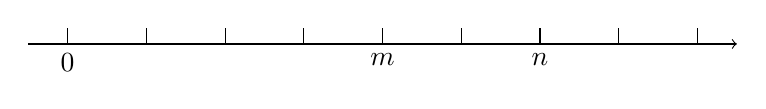
\begin{tikzpicture}
        \draw[->] (-0.5,0)--(8.5,0);
        \foreach \x in {0,1,...,8}
        \draw (\x,0.2)--(\x,0);
        \node at (0,0)[below]{0};
        \node at (4,0)[below]{$m$};
        \node at (6,0)[below]{$n$};
    \end{tikzpicture}        
    \end{center}

    显然我们可以先求出$[n,m]$,$g^m$的阶自然为$[n,m]/m=\frac{n}{(n,m)}$。下面来证明这一点:\\
    设$g^m$的阶为$N$,$(g^m)^{\frac{n}{(n,m)}}=(g^n)^{\frac{m}{(n,m)}}=e \Rightarrow N|\frac{n}{(n,m)}$;
    $(g^m)^N=g^{mN}=e \Rightarrow n|mN \Rightarrow \frac{n}{(n,m)}|\frac{m}{(n,m)}N \Rightarrow \frac{n}{(n,m)}|N$。
    故$N=\frac{n}{(n,m)}$。

    ~\\
    (2)设$gh$的阶为$N$,显然$(gh)^{mn}=e \Rightarrow N|mn$。我们只需证明$mn|N$,
    而$mn|N \Leftrightarrow m|N,n|N(\text{由于}(m,n)=1)$。
    考虑$g^n$,它的阶为$m$,又有$g^n=g^nh^n=(gh)^n$,故$g^n$的阶又等于$\frac{N}{(n,N)}$,
    所以$m=\frac{N}{(n,N)} \Rightarrow m|N$。同理$n|N$,证毕。
\end{proof}

对于定理3中的(2),自然要问$(n,m)=r \neq 1$时$gh$的阶为多少,仿效(1)可做猜想$ord(gh)=[m,n]$,
但很快能找到一个反例:$g=h=a,ord(a)=4,ord(gh)=2 \neq [4,4]$。而当$\langle g \rangle \bigcap \langle h \rangle = \{e\}$时,
仍设$ord(gh)=N$,$g^Nh^N=e \Rightarrow g^N = h^{-N}$,即只能有$g^N=h^N=e$。
则$m|N, n|N \Rightarrow [m,n]|N$,$N|[m,n]$显然,故在这种情况下$N=[m,n]$,这对我们来说已经足够。

\subparagraph{定理4} 

\subsubsection*{习题解答}
16.设$G$是有限阿贝尔群,试证:$g$对应到$g^k$是$G$的一个自同构当且仅当$k$与$|G|$互素。

由于$G$是阿贝尔群,$f_k: g \mapsto g^k$显然具有同态的性质:$f(a)f(b)=a^kb^k=(ab)^k=f(ab)$。
要使$f_k$成为自同构,我们需要它是双射。

$k$与$|G|$互素时,若$a^k=b^k$,则$(ab^{-1})^k=e \Rightarrow ord(ab^{-1}) | k$。由
$\gcd(k,|G|)=1$可得$\gcd(ord(ab^{-1}), |G|)=1$,又$ord(ab^{-1})$为$|G|$的因子,故
$ord(ab^{-1})=1 \Rightarrow ab^{-1}=e \Rightarrow a=b$,这就证明了此时$f_k$为双射。

$f_k$是双射时,考虑$G \neq \{e\}$的非平凡情况,取$e \neq g \in G$,考虑$\langle g \rangle \cong \mathbb{Z}_n$,
$n$为$g$的阶。$f_k$在$\mathbb{Z}_n$上有对应$g_k:\overline{x} \mapsto k\overline{x}$。
$k\overline{x_1} \neq k\overline{x_2} \Leftrightarrow k(x_2-x_1) \not\equiv 0 \pmod{n}$。
若$\gcd(k,n) \neq 1$,必存在$x_i,x_j, s.t. x_i-x_j=n/gcd(k,n) \Rightarrow k(x_i-x_j) \equiv 0 \pmod{n}$。
故$\gcd(k,n)=1$对所有$e \neq g \in G$均成立。应用Sylow定理可得到$\gcd(k,|G|)=1$,$k$与$|G|$互素。

~\\
可以立刻得到以下推论:
\paragraph{推论} 奇数阶阿贝尔群中每个元素$g$可表示成平方形式$g=a^2$。

\subsection{循环群}

$N\lhd G$

\subsection{正规子群、商群和同态定理}

$$a$$

\subsection{置换群}

\subsection{群在集合上的作用}



\end{document}